\documentclass[lettersize,journal]{IEEEtran}

\usepackage{cite}
\usepackage[utf8x]{inputenc} 
\usepackage{amsmath,amssymb,amsfonts}
\usepackage{amsthm}
\newtheorem{theorem}{Theorem}
\usepackage{algorithmic}
\usepackage[table,xcdraw]{xcolor}
\usepackage{float}
\usepackage{graphicx}
\usepackage[shortlabels,inline]{enumitem}
\usepackage{makecell}
\usepackage{subcaption}
\usepackage{hyperref}
\usepackage{longtable}
\usepackage{multirow}
\usepackage{url}
\usepackage{pifont}
\usepackage{textcomp}
\usepackage{ragged2e}
\usepackage[linesnumbered,ruled,vlined]{algorithm2e}
\usepackage{bm}
\usepackage{arydshln}
\usepackage{caption}
\usepackage{multirow}
\usepackage{tabularray}
\usepackage{float}
\usepackage{colortbl}
\usepackage{orcidlink}
\usepackage{booktabs}
\usepackage{pgfplots}

\pgfplotsset{compat=1.16}
\usepackage{siunitx}
\usepackage{hhline}
\usepackage[font=footnotesize,labelfont=bf,
   justification=justified,
   format=plain,skip=0pt,belowskip=0pt,aboveskip=0pt]{caption}
\usepackage{textcomp}
\usepackage[normalem]{ulem}
\usepackage{tikz}

\usepackage[capitalise,nameinlink]{cleveref}
\usepackage[normalem]{ulem}
\usepackage{tabularray}
\UseTblrLibrary{diagbox}

\usepackage{etoolbox}

\usepackage{listings}
\lstset{
    basicstyle=\tiny\ttfamily,
    breaklines=true,
    frame=single,
    numbers=left,
    numberstyle=\tiny,
    keywordstyle=\color{blue},
    commentstyle=\color{gray},
    stringstyle=\color{red},
    aboveskip=2pt,belowskip=0pt
}

% \geometry{a4paper, margin=1in}

\definecolor{phaseblue}{RGB}{0,90,170}
\definecolor{stepgreen}{RGB}{0,140,60}
\definecolor{warningred}{RGB}{180,0,40}

\usepackage{siunitx}
\usepackage{ragged2e}

\UseTblrLibrary{diagbox}
\usepackage{makecell}
\usepackage{hhline}

\newcommand*\circled[1]{\tikz[baseline=(char.base)]{
            \node[shape=circle,draw,inner sep=2pt] (char) {#1};}}
\usepackage[normalem]{ulem}


\hyphenation{op-tical net-works semi-conduc-tor IEEE-Xplore}
% updated with editorial comments 8/9/2021

\begin{document}

\title{StreamBazaar: An Auction-Based Scheduler for Multi-Tenant Streaming Clusters}

\author{Abolfazl~Younesi\IEEEauthorrefmark{1}\,\orcidlink{0009-0003-0052-6475}, (\IEEEmembership{Student, IEEE}),
Stefan~Pedratscher\IEEEauthorrefmark{1}\,\orcidlink{0000-0002-6164-880X},
Zahra~Najafabadi~Samani\IEEEauthorrefmark{1}\,\orcidlink{0000-0001-5182-9087},
Juan~Aznar~Poveda\IEEEauthorrefmark{1}\,\orcidlink{0000-0002-0879-6651},
Siavash~Razmi\IEEEauthorrefmark{1}\,\orcidlink{0009-0004-4177-0762},
Marlon~Etheredge\IEEEauthorrefmark{1}\,\orcidlink{0009-0007-3791-9378},
Philipp~Gschwandtner\IEEEauthorrefmark{1}\,\orcidlink{0000-0002-7774-0344},
Peter~Thoman\IEEEauthorrefmark{1}\,\orcidlink{0000-0002-4028-7451},
Bartosz~Balis\IEEEauthorrefmark{2}\,\orcidlink{0000-0002-3082-4209},
Thomas~Fahringer\IEEEauthorrefmark{1}\,\orcidlink{0000-0003-4293-1228}, (\IEEEmembership{Member, IEEE})
        % <-this % stops a space
\thanks{Manuscript received XX Novermber 2025; revised XX March 2026; accepted XX XXX 202X. 
Date of publication XX XXX 202X; date of current version XX XXX 202X. (Corresponding author: Abolfazl Younesi.)}
% <-this % stops a space
\thanks{\IEEEauthorrefmark{1}Department of Computer Science, University of Innsbruck, Innsbruck, Tirol, Austria.  
Emails: 
\{Abolfazl.Younesi, Stefan.Pedratscher, Zahra.Najafabadi-Samani, Juan.aznar-poveda, 
Siavash.Razmi, Marlon.Etheredge, Philipp.Gschwandtner, Peter.Thoman, Thomas.Fahringer\}@uibk.ac.at

\IEEEauthorrefmark{2}Department of Computer Science, AGH University of Krakow, Krakow, Poland.  
Email: balis@agh.edu.pl}}

% The paper headers
\markboth{IEEE Transactions on Cloud Computing,~Vol.~XX, No.~Y, November~2025}
{Younesi \MakeLowercase{\textit{et al.}}: StreamBazaar: An Auction-Based Scheduler for Multi-Tenant Streaming Clusters}


\maketitle

\begin{abstract}
Modern multi-tenant streaming clusters often waste resources due to static scheduling policies and reactive autoscaling approaches, which fail to adapt effectively to the dynamic nature of streaming workloads. Furthermore, existing systems lack the economic frameworks necessary to prioritize critical high-value streams over low-priority logs during periods of resource contention. 
We introduce \texttt{StreamBazaar}, a market-based scheduler that utilizes continuous double-auction methods to dynamically allocate resources based on real-time tenant values. \texttt{StreamBazaar} features a dynamic pricing engine that adjusts costs according to supply-demand volatility and a virtual currency system with adaptive decay that incentivizes truthful bidding while preventing resource starvation. To handle system stress, we propose a novel backpressure-aware urgency formulation that translates operator queueing signals into economic bids, coupled with a migration strategy that preserves exactly-once semantics. 
We implemented \texttt{StreamBazaar} as a pluggable scheduler for Apache Flink and evaluated it on the Chameleon Cloud testbed using real production workloads, including fraud detection and web analytics. Experimental results demonstrate that \texttt{StreamBazaar} improves resource utilization by up to $38\%$, reduces tail latency violations by up to $6.6\times$, and achieves $2.7\times$ higher throughput under peak load compared to state-of-the-art schedulers. Additionally, it lowers migration overhead by $3.3\times$.
\end{abstract}


\begin{IEEEkeywords}
Multi-Tenant Stream Processing, Resource Allocation, Scheduling, Backpressure-aware Preemption, Dynamic Pricing, Quality of Service
\end{IEEEkeywords}

\section{Introduction} \label{sec:introduction}
\IEEEPARstart{S}{tream} processing systems, such as Apache Flink, are now essential for modern data-driven applications \cite{10.1007/s10586-025-05808-w,PEDRATSCHER2025101731,schmitz2025justinhybridcpumemoryelastic}. They support everything from real-time fraud detection to IoT analytics \cite{carbone2015apache}. To reduce costs, these applications are increasingly run on shared clusters that serve multiple tenants. However, this setup brings significant challenges. Sharing resources across applications often leads to degraded service quality and unfair resource allocation \cite{8068990}.


\textcolor{blue}{\textbf{Motivation and Problem Statement.}}
\textcolor{blue}{The main challenge in multi-tenant stream processing is the gap between the continuous, fluctuating nature of streaming workloads and the rigidity of existing schedulers. Unlike batch jobs that run for a limited time \cite{10820033}, streaming applications run continuously and exhibit highly variable resource needs \cite{10.1145/2517349.2522737}. However, native schedulers in platforms such as Apache Flink, Spark Streaming, and Apache Storm rely on simple, fair-share, or static schemes that cannot adapt effectively \cite{chang2025eva,10.1145/3267809.3267832, lian2023conttune, 10.1145/2517349.2522737,younesi2025autostreampipellmassistedautomatic}.}

\textcolor{blue}{While recent efforts have introduced adaptive autoscaling to address these fluctuations, they predominantly rely on reactive performance metrics \cite{chen2025oceanus,wang2025capsys,kalavri2018three,10.1145/3267809.3267832,ntouni2024talos}. A critical pain point is that these approaches lack an explicit economic framework necessary to prioritize critical high-value streams over low-priority logs during periods of resource contention. Consequently, when cluster resources are saturated, these systems often treat all workloads indistinguishably, causing significant inefficiencies, severe backpressure, and high latency \cite{lian2023conttune}. Without an economic mechanism, tenants cannot communicate the business value of their workloads. By treating resources as a continuous commodity market, an auction-based economic mechanism naturally solves this limitation, allowing the system to dynamically translate workload urgency into economic bids and prioritize critical applications effectively.}

\textbf{Solution.} We present \texttt{StreamBazaar}, a novel resource-pricing and auction-based scheduler that introduces market dynamics to multi-tenant streaming clusters. Our main idea is that resources should be viewed as a continuous commodity market rather than as separate allocation units. \texttt{StreamBazaar} employs a continuous double-auction mechanism in which tenants submit bids indicating their resource requirements and the maximum amount they are willing to pay. These bids are updated in real-time as stream characteristics change. The system features a pricing engine that looks at several factors: current cluster usage, historical demand patterns, and stream-specific metrics such as ingestion rate and processing complexity. To ensure the process is fair and avoid resource shortages, we implement a virtual currency system. Tenants receive periodic budget allocations based on their organizational priorities and past usage. A decay mechanism encourages immediate resource use instead of hoarding. When resource conflicts arise, \texttt{StreamBazaar}'s strategy for handling backpressure carefully moves operators while keeping processing accurate, using checkpoint coordination to limit disruption to downstream operators. The scheduler continually optimizes resource allocation using an online algorithm that resolves the winner-determination problem in less than a second. This ensures that resources go to tenants who value them the most while still maintaining quality of service guarantees.

\textbf{Contributions.} This paper makes the following contributions:

\begin{itemize}[leftmargin=*,wide]
    \item[\textbf{C1)}] We introduce the first \emph{continuous double-auction mechanism} for multi-tenant stream processing, explicitly tailored to the dynamics of streaming workloads with a pricing model that captures stream-specific characteristics, including rate variations, processing complexity, and latency requirements.

    
    \item[\textbf{C2)}] We develop a \emph{backpressure-aware urgency formulation} that translates operator queueing stress into bidding signals, and pair it with a lightweight preemption and migration strategy that preserves exactly-once semantics while minimizing disruption to end-to-end latency.
    
    \item[\textbf{C3)}] We propose a \emph{virtual currency system with adaptive decay}, which both incentivizes sustained bidding discipline and prevents budget hoarding, thereby ensuring long-term fairness and avoiding starvation across tenants.
    
    \item[\textbf{C4)}] We implement \texttt{StreamBazaar}\footnote{\url{https://github.com/Anonymous0-0paper/Streambazaar}} as a pluggable scheduler for Apache Flink. Through extensive experiments on the Chameleon Cloud with diverse real-world streaming applications, we show that \texttt{StreamBazaar} gains up to $38\%$ higher resource utilization, $6.6\times$ fewer tail-latency violations, $2.7\times$ higher throughput, and $3.3\times$ lower migration overhead compared to state-of-the-art schedulers.
\end{itemize}


\textbf{Paper Organization.} 
The remainder of this paper is organized as follows. 
Section~\ref{sec:related} reviews existing works.
Section~\ref{sec:architecture} presents the design of \texttt{StreamBazaar},
Section~\ref{sec:scheduling_algorithm} describes the integration of \texttt{StreamBazaar},
Section~\ref{sec:performance} evaluates \texttt{StreamBazaar}.
Finally, Section~\ref{sec:conclusion} concludes the paper and outlines future research directions.


\section{Related Work}
\label{sec:related}
Resource allocation in multi-tenant stream processing has been extensively studied. Early approaches focused on static resource partitioning and slot-based scheduling, as seen in Flink’s default scheduling mechanism~\cite{carbone2015apache,10.1007/s10586-025-05808-w}, but such approaches often led to underutilization and poor adaptability to workload fluctuations. 

To overcome these limitations, adaptive autoscaling has received significant attention. \textcolor{blue}{Systems like Henge \cite{10.1145/3267809.3267832} utilize utility-based SLOs to reallocate resources dynamically, while DS2 \cite{kalavri2018three} and TALOS \cite{ntouni2024talos} employ control-theoretic models and task-level monitoring for rapid scaling decisions. Recent efforts like CAPSys \cite{wang2025capsys} further optimize this through contention-aware placement search. While these systems improve elasticity, they are fundamentally metric-driven and lack explicit economic mechanisms. Crucially, when cluster capacity is saturated, these approaches often default to indiscriminate load shedding or equal-share throttling, failing to protect high-priority tenants from ``noisy neighbors'' running low-value workloads.}

Auction-based scheduling methods have gained interest because they can balance conflicting goals in changing environments. However, their use in streaming clusters is still limited, particularly when considering workload-specific factors such as rate variability, backpressure, and stateful operator migration. Avni et al.~\cite{avni2024auction} presented a decentralized auction-based scheduling framework for sequential decision making. The scheduler assigns budgets to competing policies using bidding mechanisms that ensure both fairness and flexibility across multiple objectives. Similarly, Wu et al.~\cite{wu2012auction} used auction-based mechanisms to optimize block scheduling and incentive alignment in P2P video-on-demand streaming, thereby maximizing social welfare. However, these general-purpose mechanisms typically assume discrete, independent tasks and do not account for the continuous, unbounded nature of data streams, in which preemption costs vary dynamically with the operator's state size.

Another important aspect of resource management in streaming systems is the pricing strategy. Hao et al.~\cite{hao2023evolution} studied the development of data pricing in cloud and streaming infrastructures. They highlighted future directions for making money from data-driven infrastructure. Wang et al.~\cite{wang2022analysis} explored the impact of fairness concerns on live streaming pricing, showing that heterogeneous user preferences require adaptive, fair pricing mechanisms in large-scale streaming.

Beyond cluster-level autoscaling and pricing, recent work in computational economics and queueing-based scheduling also informs the design of resource-allocation mechanisms relevant to streaming systems. Lahaie and Lubin~\cite{lahaie2025iterative} introduced a linear-programming framework for constructing iterative Vickrey (VCG) auctions using universal competitive equilibrium prices, achieving truthful and efficient allocations with a single price path. Their formulation significantly reduces demand-query complexity compared to product-mix auctions, but it assumes a static market and does not address continuously evolving stream workloads, backpressure dynamics, or the cost of migrating stateful operators in distributed dataflow engines.
At the systems level, Justin~\cite{schmitz2025justinhybridcpumemoryelastic} proposes a hybrid CPU/memory auto-scaler for Apache Flink that jointly adjusts operator parallelism and RocksDB-managed memory. By decoupling CPU and memory provisioning, Justin achieves lower resource consumption than DS2 on Nexmark workloads. However, its decisions are purely metric-driven without incorporating tenant utility, pricing, or budget-based prioritization. Moreover, it is evaluated in a single-tenant setting and does not address multi-tenant contention or economic allocation.
In a different direction, Hu and Smith’s Softpressure algorithm~\cite{hu2019softpressurescheduledrivenbackpressurealgorithm} blends backpressure from queueing theory with schedule-driven control to stabilize queues in large networks, yielding substantial delay reductions in traffic control tasks. Although conceptually related to backpressure-aware operator scheduling, Softpressure lacks an economic layer, does not model heterogeneous compute/memory/network resources, and operates in domains without state migration or exactly-once semantics.

\textbf{Position of StreamBazaar.} Overall, while prior work has advanced elasticity, contention management, and placement strategies, these approaches either lack economic incentives, ignore multi-tenant prioritization under scarcity, or operate under abstractions that do not capture stateful stream-processing constraints. A gap remains in unifying economic principles with the unique demands of stream processing, motivating the design of auction-based schedulers, such as \texttt{StreamBazaar}. Our approach bridges this gap by directly translating low-level backpressure signals into economic urgency, ensuring that scarcity is managed through market valuation rather than arbitrary throttling.

\section{System Model}
\label{sec:architecture}

% \subsection{System Overview}
% \label{subsec:system_overview}
\texttt{StreamBazaar} operates as a pluggable scheduling layer that interfaces between streaming applications and cluster resource managers. \textcolor{blue}{To illustrate the lifecycle of a scheduling decision, Figure~\ref{fig:architecture} maps the data flow across five core components: (i) the \textit{Tenant Manager} receives application graphs and resource requirements as inputs, outputting validated bid bundles (see Sections~\ref{subsec:tenant_model} and \ref{subsec:currency_system}), (ii) the \textit{Pricing Engine} synthesizes historical demand and current cluster utilization to output dynamic base prices (see Section~\ref{subsec:pricing_engine}), (iii) the \textit{Auction Orchestrator} evaluates incoming bids against these prices to resolve the winner determination problem based on backpressure urgency (see Section \ref{subsec:auction_mechanism}), (iv) the \textit{Resource Allocator} executes the physical mapping of winning bids to cluster nodes (see Section \ref{subsec:online_allocation}), and (v) the \textit{Migration Coordinator} manages operator preemption, utilizing synchronization barriers as input to output consistent state transfers that preserve exactly-once semantics (see Section~\ref{subsec:state_migration}).}

\begin{figure}[t]
\centering
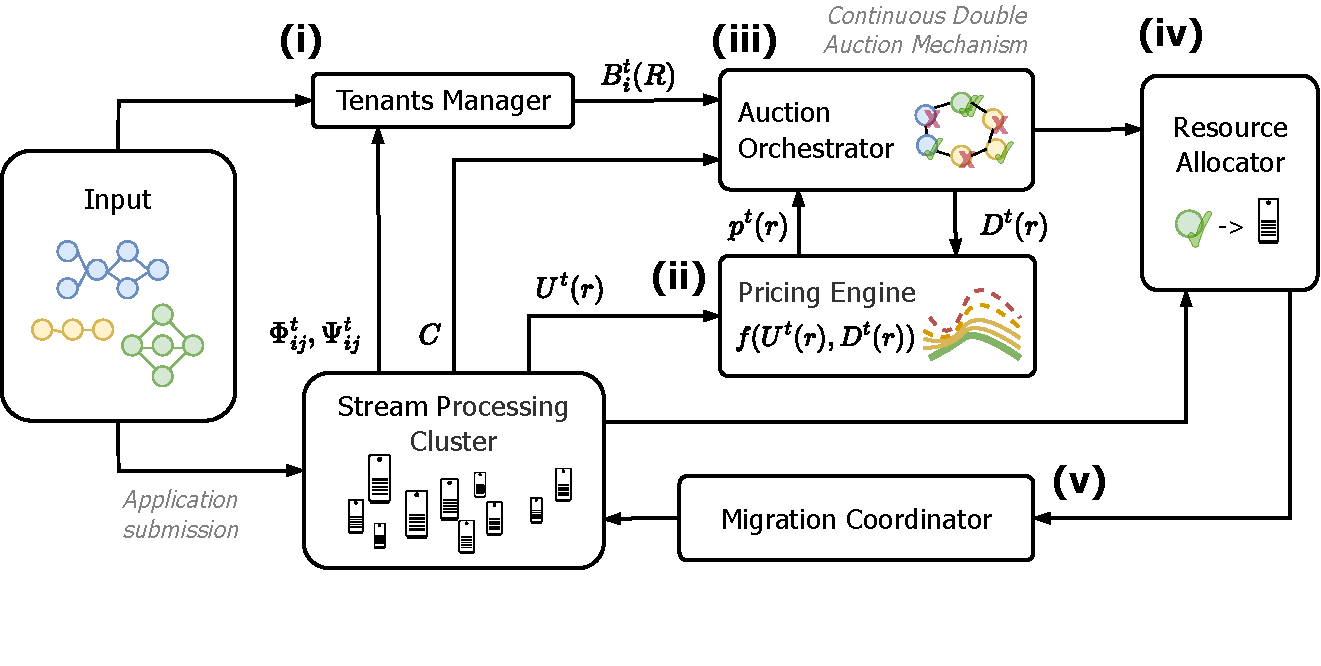
\includegraphics[width=\columnwidth]{Figures/arch.drawio.pdf}
\caption{\texttt{StreamBazaar} architecture overview including core components.}
\label{fig:architecture}
\end{figure}



\subsection{Tenant Manager Model}
\label{subsec:tenant_model}


Each tenant $i \in \mathcal{T}$ submits a streaming application represented as a DAG $G_i = (V_i, E_i)$, where vertices $V_i$ represent operators and edges $E_i$ denote data streams between operators. For each operator $s_{ij} \in \mathcal{S}_i$, tenants specify resource requirements as a vector $\mathbf{r}_{ij} = \langle c_{ij}, m_{ij}, n_{ij} \rangle$ representing CPU cores, memory, and network bandwidth, respectively. 


The actual resource consumption of an operator depends on its input rate and processing complexity:
\begin{equation}
\label{eq:actual_resource}
\mathbf{r}_{ij}^{\text{actual}}(t) = \mathbf{r}_{ij}^{\text{base}} \cdot \left(1 + \rho_{ij} \cdot \frac{\lambda_{ij}(t)}{\lambda_{ij}^{\text{ref}}}\right)
\end{equation}
where $\mathbf{r}_{ij}^{\text{base}}$ represents the baseline resource requirement, $\lambda_{ij}(t)$ is the current input rate, $\lambda_{ij}^{\text{ref}}$ is the reference input rate used for baseline measurement, and $\rho_{ij} \in [0, 1]$ captures the operator's sensitivity to input rate variations.


\subsubsection{Resource Request} 
Tenants request resources as bundles $\mathbf{R} = \{r_1, r_2, ..., r_k\}$, where each $r_i \in \mathcal{R}$ represents a resource type and quantity pair. Each bundle encapsulates an operator's complete requirements, enabling atomic allocation. This per-operator bundling simplifies bidding: tenants submit bid sets $\mathcal{B}_i^t$ with one bid per operator.
\subsection{Virtual Currency System}
\label{subsec:currency_system}

To ensure fairness and prevent resource starvation, we implement a virtual currency system with periodic allocations and strategic decay mechanisms in \texttt{StreamBazaar}.

\subsubsection{Currency Allocation}
\label{ssub:currency_allocation}

Each tenant receives a periodic currency injection based on priorities and historical usage:
\begin{equation}
\label{eq:currency_allocation}
\omega_i^{t+\Delta} = \omega_i^t \cdot (1 - \gamma) + A_i \cdot \left(\alpha_i + \eta \cdot \frac{U_i^{\text{avg}}}{U^{\text{total}}}\right)
\end{equation}
where $\gamma$ is the decay rate preventing hoarding, $A_i$ is the base allocation, $\alpha_i$ represents organizational priority, and the second term rewards efficient resource utilization based on average usage $U_i^{\text{avg}}$. We typically set $\gamma = 0.05$, allowing 95\% of unspent currency to carry over.

\subsubsection{Strategic Bidding Incentives}
\label{ssub:bidding_incentives}

To encourage truthful bidding, we implement a second-price mechanism where winning tenants pay the minimum amount needed to win:
\begin{equation}
\label{eq:payment}
\text{Payment}_i = \min\{b_k : b_k > b_{-i}^{\max}\}
\end{equation}
where $b_{-i}^{\max}$ is the highest competing bid that would win if tenant $i$ were absent. This approximates Vickrey-Clarke-Groves (VCG) \cite{vickrey1961counterspeculation,clarke1971multipart,lahaie2025iterative} incentives in our budget-constrained combinatorial setting, making truthful valuation reporting a near-dominant strategy.

\subsubsection{Mechanism Analysis}
\label{ssub:mechanism_analysis}

To address the theoretical stability of the auction under budget constraints, we analyze the tenant's utility maximization problem. While standard VCG guarantees dominant-strategy truthfulness only in the absence of budget limits, we prove that \texttt{StreamBazaar}'s combination of backpressure-based urgency and price smoothing makes truthful bidding an asymptotically dominant strategy.

\begin{theorem}[Asymptotic Truthfulness under Backpressure]
Given the resource price smoothing function in Eq.~\ref{eq:price_update} and the exponential urgency factor in Eq.~\ref{eq:urgency_factor}, truthful bidding $b_i^t = \min(v_{ij}, \omega_i)$ is a strictly dominant strategy as the upstream queue length $q_{ij}^t$ approaches the capacity $q_{ij}^{\max}$.
\end{theorem}

\begin{proof}
Let $u_i(b_i, b_{-i})$ be the utility of tenant $i$ given their bid $b_i$ and opposing bids $b_{-i}$. In our second-price setting (Eq.~\ref{eq:payment}), the utility is defined as $u_i = v_{ij} - b_{-i}^{\max}$ if the bid wins, and $0$ otherwise. A tenant might attempt "bid shading" (submitting $b_i' < v_{ij}$) to manipulate the aggregate demand $D^t(r)$ (Eq.~\ref{eq:demand}), aiming to lower the future base price $p^{t+1}(r)$.
However, the price update function (Eq.~\ref{eq:price_update}) incorporates a smoothing parameter $\theta$. The marginal gain from shading is bounded linearly by $(1-\theta)$. Conversely, the cost of losing a bid (preemption) results in an increase in queue length $q_{ij}$. According to Eq.~\ref{eq:urgency_factor}, the urgency factor $\phi_{ij}^t$ grows exponentially with $q_{ij}$.

Let $\Delta U_{\text{save}}$ be the utility gained from price reduction and $\Delta U_{\text{delay}}$ be the utility lost due to increased latency/backpressure. As $q_{ij} \to q_{ij}^{\max}$, the urgency gradient $\frac{\partial \phi}{\partial q}$ dominates the price gradient $\frac{\partial p}{\partial D}$. Consequently:
\begin{equation}
\lim_{q_{ij} \to q_{ij}^{\max}} \frac{\Delta U_{\text{delay}}}{\Delta U_{\text{save}}} \to \infty
\end{equation}
Thus, any strategy $b_i < v_{ij}$ increases the risk of resource starvation and subsequent backpressure penalties, yielding lower long-term utility than the truthful strategy.
\end{proof}


\subsection{Dynamic Pricing Engine}
\label{subsec:pricing_engine}

The pricing engine computes resource prices that reflect current cluster conditions and historical demand patterns. We model resource pricing as a continuous function that adapts to supply-demand imbalances while preventing price volatility that could destabilize bidding strategies.
\begin{table}
\centering
\caption{Notation used throughout the paper.}
\label{table:notation}
\resizebox{\linewidth}{!}{%
\begin{tabular}{ll} 
\hline
\rowcolor[rgb]{0.816,0.816,0.816} \textbf{Symbol} & \textbf{Description} \\ 
\hline
$\mathcal{T}$ & Set of tenants \\
$\mathcal{R}$ & Set of resource types (CPU, memory, network) \\
$\mathbf{r}_{ij}=\langle c_{ij}, m_{ij}, n_{ij}\rangle$ & Nominal resource request for operator $j$ of tenant $i$ \\
$\mathbf{r}_{ij}^\text{base}$ & Baseline resource requirement for $s_{ij}$ at reference rate \\
$\lambda_{ij}(t)$, $\lambda_{ij}^\text{ref}$ & Current and reference input rates for $s_{ij}$ \\
$\rho_{ij}\in[0,1]$ & Sensitivity of $s_{ij}$ to input-rate variation \\
$\mathbf{R}_{ij}\subseteq \mathcal{R}$ & \textit{Bundle} proposed for operator $j$ (typed quantities) \\
$\mathbf{R}_i=\{\mathbf{R}_{ij}\}_j\in\mathcal{S}_i$ & Tenant $i$'s set of bundles (possibly grouped atomically) \\
$B_i^t(\mathbf{R}_{ij})$ & Tenant $i$'s valuation (bid) for bundle $\mathbf{R}_{ij}$ at time $t$ \\
$p^t(r)$ & Base price of resource type $r$ at time $t$ \\
$U^t(r)$, $C(r)$ & Utilization and total capacity of resource $r$ \\
$D^t(r)$ & Aggregate demand (bid-weighted) for resource $r$ at time $t$ \\
$\omega_i$ & Tenant $i$'s \textit{credit} balance (virtual tokens) \\
$\alpha_i$ & Priority weight for tenant $i$ \\
$q_{ij}^t$, $q_{ij}^{\max}$ & Queue length and capacity upstream of operator $j$ \\
$\phi_{ij}^t$ & Urgency factor derived from backpressure at $s_{ij}$ \\
$\tau_{ij}$, $Q_i^\text{latency}$ & Latency SLO and required success probability \\
$\beta,\gamma,\zeta,\kappa,\mu,\eta,\theta$ & Control parameters (defined in context) \\
$\Delta$ & Auction interval duration \\
\hline
\end{tabular}
}
\end{table}
The base price for resource $r$ at time $t$ follows an exponential smoothing model with demand-driven adjustments \cite{agrawal2024dynamic}:
\begin{equation}
\label{eq:price_update}
p^t(r) = \theta \cdot p^{t-1}(r) + (1-\theta) \cdot p^{\text{spot}}(r) \cdot f(U^t(r), D^t(r))
\end{equation}

where $\theta \in [0,1]$ is the smoothing parameter, $p^{\text{spot}}(r)$ represents the spot price computed from current bids, and $f(U^t(r), D^t(r))$ is an adjustment function based on utilization $U^t(r)$ and demand $D^t(r)$. To ensure the price reflects the true marginal value of resources, we define the spot price $p^{\text{spot}}(r)$ as the auction's clearing price. Specifically, it corresponds to the bid density of the lowest successful bid that clears the market for resource $r$:
\begin{equation}
\label{eq:spot_price}
p^{\text{spot}}(r) = \min_{(i,j) \in \text{Winners}} \left( \frac{B_i^t(\mathbf{R}_{ij})}{\|\mathbf{R}_{ij}\|_2} \right)
\end{equation}
This definition ensures that the baseline price tracks the effective clearing price established by the most competitive marginal winner.

The demand $D^t(r)$ for resource $r$ at time $t$ is computed from the aggregate bid volume across all tenants:
\begin{equation}
\label{eq:demand}
D^t(r) = \sum_{i \in \mathcal{T}} \sum_{\mathbf{R} \in \mathcal{B}_i^t} B_i^t(\mathbf{R}) \cdot \mathbb{I}[r \in \mathbf{R}]
\end{equation}
where $\mathcal{B}_i^t$ represents tenant $i$'s bid set at time $t$, and $\mathbb{I}[r \in \mathbf{R}]$ is an indicator function that equals 1 if resource $r$ is included in bundle $\mathbf{R}$. This formulation captures the total economic demand by aggregating all bids that include resource $r$, weighted by their monetary valuations.

The adjustment function incorporates both current utilization and predicted demand:
\begin{equation}
\label{eq:adjustment_function}
\resizebox{0.89\columnwidth}{!}{$
f(U^t(r), D^t(r)) =
\begin{cases}
1 + \kappa \left(U^t(r) - U^{\text{target}}\right)^2 + \eta \frac{D^t(r)}{C(r)},
& \text{if } U^t(r) > U^{\text{target}}, \\[1ex]
1 - \mu \left(U^{\text{target}} - U^t(r)\right) \cdot \left(1 - \frac{D^t(r)}{C(r)}\right),
& \text{if } U^t(r) \leq U^{\text{target}}
\end{cases}
$}
\end{equation}
where  $U^{\text{target}}$ is the target utilization, usually set at 0.8 \cite{10.1145/3303849}. The variable $\kappa$ controls how quickly prices rise when utilization is high. The variable $\mu$ determines the speed of price drops during low utilization. The function $C(r)$ represents the total capacity of resource $r$. The variable $\eta$ measures how sensitive demand is to changes. The ratio $\frac{D^t(r)}{C(r)}$ indicates the pressure on demand. If demand goes above capacity, prices rise more sharply. When demand is low compared to capacity, prices drop more quickly.
\textcolor{blue}{The intuition behind this Eq.~\ref{eq:adjustment_function} is structural stabilization: it intentionally ensures that prices scale quadratically during severe contention (when $U^t > U^{\text{target}}$) to rapidly suppress excessive demand and force resource release. Conversely, prices decay linearly during under-utilization to economically incentivize workloads to scale up and consume idle resources.}

\subsection{Auction Orchestrator}
\label{subsec:auction_mechanism}
\texttt{StreamBazaar} implements a continuous double auction running at $\Delta$-second intervals (typically 1s), where tenants act as both buyers (bidding for resources) and sellers (releasing underutilized resources). This balances responsiveness with computational overhead. While the auction intervals are discrete, the economy operates as an open system. The orchestrator acts as the clearinghouse, managing the flow of virtual currency not only through payments but also through strategic refunds.

\subsubsection{Bid Formulation}
\label{ssub:bid_formulation}
Each tenant $i$ submits a bid function $B_i^t$ that maps resource bundles to valuations. For a resource bundle $\mathbf{R} = \{r_1, r_2, ..., r_k\}$, the bid is computed as:
\begin{equation}
\label{eq:bid_function}
B_i^t(\mathbf{R}) = \sum_{j \in \mathcal{S}_i} v_{ij}(\mathbf{R}_j) \cdot \phi_{ij}^t \cdot \psi_{ij}^t
\end{equation}
where $v_{ij}(\mathbf{R}_j)$ is the base valuation for resources allocated to operator $j$, $\phi_{ij}^t$ is a urgency factor based on backpressure, and $\psi_{ij}^t$ represents the latency sensitivity.
The latency sensitivity $\psi_{ij}^t$ is derived directly from the operator’s latency service-level objective (SLO) $\tau_{ij}$ and its recent latency performance. Specifically, it is computed as:
\begin{equation}
\label{eq:latency_sensitivity}
\psi_{ij}^t = 
\begin{cases}
1 + \varrho  \cdot \left(1 - \frac{\text{latency}_{ij}^t}{\tau_{ij}}\right)^{-1}, & \text{if } \text{latency}_{ij}^t < \tau_{ij} \\
1 + \varrho  \cdot \frac{\text{latency}_{ij}^t}{\tau_{ij}}, & \text{otherwise}
\end{cases}
\end{equation}
where $\text{latency}_{ij}^t$ is the observed end-to-end latency of operator $j$ at time $t$, $\tau_{ij}$ is its SLO threshold, and $\varrho  > 0$ is a tunable parameter that controls the steepness of the sensitivity curve. The use of inverse scaling below the SLO prevents over-provisioning for already-compliant workloads.
The urgency factor increases exponentially with backpressure:
\begin{equation}\label{eq:urgency_factor}
\phi_{ij}^t = \exp\left(\beta \cdot \frac{q_{ij}^t}{q_{ij}^{\max}}\right)
\end{equation}
where $q_{ij}^t$ is the current queue length upstream of operator $j$, $q_{ij}^{\max}$ is the maximum queue capacity, and $\beta$ controls the sensitivity to backpressure.
\textcolor{blue}{Eq.~\ref{eq:urgency_factor} inherently links economic valuation to application health. Rather than relying on manual, static bids, the urgency factor ($\phi_{ij}^t$) acts as a critical, automated safety valve. As an operator experiences backpressure (queue buildup), its bidding power scales exponentially.}
\textcolor{blue}{This guarantees that stressed operators automatically outbid healthy ones, securing the resources necessary to process backlogs and preventing cascading cluster failures without tenant intervention.}

\textbf{Seller Incentives (Resource Release).} Tenants implicitly participate as sellers by releasing allocated resources prior to lease expiration. To align seller incentives with system liquidity, we implement a buy-back mechanism where a releasing tenant $i$ receives a pro-rated refund to their virtual balance $\omega_i$:
\begin{equation}
\omega_i \leftarrow \omega_i + \text{Payment}_i \cdot \frac{T_{\text{remain}}}{T_{\text{lease}}}
\end{equation}
This encourages tenants to relinquish underutilized resources immediately rather than hoarding them, thereby increasing the supply available for high-urgency bids.

\subsubsection{Winner Determination}
\label{ssub:winner_determination}

The winner determination problem seeks to maximize social welfare while respecting resource constraints:
\begin{align}
\max_{\mathbf{X}} \quad & \sum_{i \in \mathcal{T}} \sum_{j \in \mathcal{S}_i} B_i^t(\mathbf{R}_j) \cdot x_{ij} \\
\text{s.t.} \quad & \sum_{i \in \mathcal{T}} \sum_{j \in \mathcal{S}_i} r_{ijk} \cdot x_{ij} \leq C_k, \quad \forall k \in \mathcal{R} \\
& \sum_{j \in \mathcal{S}_i} B_i^t(\mathbf{R}_j) \cdot x_{ij} \leq \omega_i, \quad \forall i \in \mathcal{T} \\
& x_{ij} \in \{0, 1\}, \quad \forall i \in \mathcal{T}, j \in \mathcal{S}_i
\end{align}
where $x_{ij}$ indicates whether operator $j$ of tenant $i$ wins its bid, $C_k$ is the capacity of resource $k$, and the second constraint ensures tenants don't exceed their virtual currency balance $\omega_i$.
\textcolor{blue}{This formulation ensures that total allocated resources do not exceed cluster capacity ($C_k$) and that tenants cannot exceed their available virtual credit ($\omega_i$), ultimately yielding a binary placement matrix ($x_{ij}$) that assigns resources to the highest-valued streams.}

\subsection{Quality of Service Enforcement}
\label{subsec:qos_enforcement}

\texttt{StreamBazaar} enforces quality of service requirements through constraint-based allocation and penalty mechanisms. For each operator with latency constraint $\tau_{ij}$, we ensure:

\begin{equation}
\mathbb{P}[\text{latency}_{ij} \leq \tau_{ij}] \geq Q_i^{\text{latency}}
\end{equation}

where $Q_i^{\text{latency}}$ is the required latency SLA. Violations trigger automatic bid adjustments:
\begin{equation}
B_i^{t+1}(\mathbf{R}) = B_i^t(\mathbf{R}) \cdot \left(1 + \zeta \cdot \frac{\text{violations}_i^t}{\text{total}_i^t}\right)
\end{equation}
where $\zeta$ controls the aggressiveness of bid increases in response to SLA violations. This system-enforced adjustment incentivizes tenants to bid sufficiently to meet SLAs. \textcolor{blue}{We have enforced this system penalty mechanism, which automates SLA compliance: if an application misses its latency targets, the system artificially inflates its bid for the next auction round ($\zeta$), ensuring it acquires sufficient resources to recover without requiring manual intervention from the tenant.}


\section{\texttt{StreamBazaar} Implementation}
\label{sec:scheduling_algorithm}

\subsection{Online Resource Allocation}
\label{subsec:online_allocation}

\texttt{StreamBazaar}'s scheduling algorithm operates online, making allocation decisions at each auction interval without knowledge of future bids. 
The Algorithm~\ref{alg:allocation} operates in two main phases. 

\begin{algorithm}[h]
\SetAlgoLined
\SetAlgoNoEnd
\scriptsize
\KwIn{Current bids $\mathcal{B}^t$, Resource capacity $\mathcal{C}$, Virtual balances $\Omega$}
\KwOut{Allocation matrix $\mathbf{X}$, Preemption set $\mathcal{P}$}
\SetKwFunction{FValidate}{ValidateBids}
\SetKwFunction{FCompute}{ComputeEfficiency}
\SetKwFunction{FDetermine}{DetermineWinners}
\SetKwFunction{FPreempt}{SelectPreemption}

\tcc{\textcolor{phaseblue}{\textbf{Phase 1: Validation of incoming bids}}}
$\mathcal{B}^{\text{valid}} \leftarrow \emptyset$\;
\ForEach{$b_i \in \mathcal{B}^t$}{
    \If{\FValidate{$b_i, \omega_i$}}{\label{line:validate}
        $e_i \leftarrow$ \FCompute{$b_i$}\tcp*{\textbf{Compute bid efficiency}}\label{line:efficiency}
        $\mathcal{B}^{\text{valid}} \leftarrow \mathcal{B}^{\text{valid}} \cup \{(b_i, e_i)\}$\;
    }
}

\tcc{\textcolor{phaseblue}{\textbf{Phase 2: Greedy allocation by efficiency ranking}}}
$\mathcal{B}^{\text{sorted}} \leftarrow$ \texttt{Sort}($\mathcal{B}^{\text{valid}}$, key=$e_i$, order=DESC)\;\label{line:sort}
$\mathbf{X} \leftarrow \mathbf{0}$\;
$\mathcal{C}^{\text{avail}} \leftarrow \mathcal{C}$\;

\ForEach{$(b_i, e_i) \in \mathcal{B}^{\text{sorted}}$}{\label{line:greedy-start}
    \If{$\mathbf{r}_i \leq \mathcal{C}^{\text{avail}}$}{\label{line:capacity-check}
        $\mathbf{X}[i] \leftarrow 1$\;
        $\mathcal{C}^{\text{avail}} \leftarrow \mathcal{C}^{\text{avail}} - \mathbf{r}_i$\;
        $\omega_i \leftarrow \omega_i - \text{CalculatePayment}(i, \mathcal{B}^{\text{sorted}})$\tcp*{\textbf{Deduct payment}}\label{line:payment}
    }
    \Else{
        \tcp{\textbf{Check if preemption is beneficial}}
        $\mathcal{P}_{\text{cand}} \leftarrow$ \FPreempt{$b_i, \mathbf{X}, \mathcal{B}^{\text{valid}}$}\;\label{line:preempt-check}
        \If{$\sum_{j \in \mathcal{P}_{\text{cand}}} b_j < b_i$}{\label{line:preempt-condition}
            $\mathcal{P} \leftarrow \mathcal{P} \cup \mathcal{P}_{\text{cand}}$\;
            \ForEach{$j \in \mathcal{P}_{\text{cand}}$}{
                $\mathbf{X}[j] \leftarrow 0$\;
                $\mathcal{C}^{\text{avail}} \leftarrow \mathcal{C}^{\text{avail}} + \mathbf{r}_j$\;
            }
            $\mathbf{X}[i] \leftarrow 1$\;
            $\mathcal{C}^{\text{avail}} \leftarrow \mathcal{C}^{\text{avail}} - \mathbf{r}_i$\;
        }
    }
}\label{line:greedy-end}
\Return{$\mathbf{X}, \mathcal{P}$}\;
\caption{\texttt{StreamBazaar} Online Allocation}
\label{alg:allocation}
\end{algorithm}
The algorithm first validates each bid (Line~\ref{line:validate}) to ensure that it does not exceed the tenant's virtual currency balance~$\omega_i$, preventing overbidding. \textcolor{blue}{This validation also enforces currency limits to maintain macroeconomic stability and ensure tenants cannot spend beyond their allocated budgets.} For each valid bid, the efficiency metric (Line~\ref{line:efficiency}) is computed as:
\begin{equation}
e_i =
\underbrace{\frac{b_i}{\|\mathbf{r}_i\|_2}}_{\text{bid density}} \cdot
\underbrace{\phi_i^t}_{\text{urgency}} \cdot
\underbrace{\min\left(1, \frac{\omega_i}{\bar{\omega}}\right)}_{\text{spending incentive}}
\end{equation}
The first term represents bid density (value per unit of resource), $\phi_i^t$ denotes the backpressure-derived urgency factor, and the final term discourages tenants from hoarding currency. \textcolor{blue}{Thus, the efficiency metric acts as a dynamic priority score that boosts congested operators while encouraging active market participation.}
After computing efficiencies, bids are sorted in descending order (Line~\ref{line:sort}) to produce a prioritized list $\mathcal{B}^{\text{sorted}}$. \textcolor{blue}{Rather than solving the NP-hard multidimensional knapsack problem exactly, the algorithm uses a greedy approximation based on this score, enabling low-latency scheduling in streaming environments.} The allocation matrix $\mathbf{X}$ is initialized to zero and the available capacity $\mathcal{C}^{\text{avail}}$ is set to the total cluster capacity.
The algorithm then processes each bid sequentially (Lines~\ref{line:greedy-start}-\ref{line:greedy-end}). If the requested resources $\mathbf{r}_i$ fit within $\mathcal{C}^{\text{avail}}$ (Line~\ref{line:capacity-check}), the bid is accepted, the allocation matrix is updated ($\mathbf{X}[i] \leftarrow 1$), capacity is reduced, and the tenant’s balance is charged according to the second-price rule defined in Eq.~\ref{eq:payment}.

If resources are insufficient, the algorithm invokes \texttt{SelectPreemption} (Line~\ref{line:preempt-check}) to identify preemption candidates. Preemption occurs only if the incoming bid exceeds the combined value of the displaced operators (Line~\ref{line:preempt-condition}), thereby improving overall social welfare. \textcolor{blue}{Thus, preemption is triggered only when replacing existing allocations increases system-wide efficiency.}



\subsection{Backpressure-Aware Preemption}
\label{subsec:backpressure_preemption}

When resource contention occurs, \texttt{StreamBazaar} must carefully select which operators to preempt while minimizing disruption to running streams. Algorithm~\ref{alg:preemption} details our backpressure-aware preemption strategy.
This process starts by identifying potential candidates for preemption (Line \ref{line:candidates}). These candidates are currently allocated operators with bid values lower than the incoming bid $b_{\text{new}}$, making them suitable for preemption. The algorithm initializes empty sets for the final preemption selection $\mathcal{P}$ and the migration plan $\mathcal{M}$ that will manage the actual operator movements.
\begin{algorithm}
\SetAlgoLined
\SetAlgoNoEnd\scriptsize
\KwIn{Candidate bid $b_{\text{new}}$, Current allocations $\mathbf{X}$, Operator graph $G$}
\KwOut{Preemption set $\mathcal{P}$, Migration plan $\mathcal{M}$}
\SetKwFunction{FBackpressure}{ComputeBackpressure}
\SetKwFunction{FDownstream}{GetDownstream}
\SetKwFunction{FCheckpoint}{EstimateCheckpointTime}
\SetKwFunction{FImpact}{EstimateImpact}
\tcc{\textcolor{phaseblue}{\textbf{Phase 1: Identify preemption candidates}}}
$\mathcal{P}_{\text{pot}} \leftarrow \{i : \mathbf{X}[i] = 1 \land b_i < b_{\text{new}}\}$\;\label{line:candidates}
$\mathcal{P},\mathcal{M} \leftarrow \emptyset, \emptyset$\;
\tcc{\textcolor{phaseblue}{\textbf{Phase 2: Evaluate backpressure impact}}}
\ForEach{$i \in \mathcal{P}_{\text{pot}}$}{\label{line:bp-start}
    $bp_i \leftarrow$ \FBackpressure{$i, G$}\;\label{line:bp-compute}
    $\mathcal{D}_i \leftarrow$ \FDownstream{$i, G$}\;\label{line:downstream}
    $impact_i \leftarrow bp_i \cdot |\mathcal{D}_i|$\;\label{line:impact}
    \If{HasState($i$)}{\tcp{\textbf{Check if operator has recoverable state}}\label{line:state-check}
        $t_{\text{ckpt}} \leftarrow$ \FCheckpoint{$i$}\;\label{line:checkpoint-time}
        $impact_i \leftarrow impact_i \cdot (1 + \xi \cdot t_{\text{ckpt}})$\;\label{line:adjust-impact}
    }
}
\tcc{\textcolor{phaseblue}{\textbf{Phase 3: Select minimum impact set}}}
$\mathcal{P}_{\text{sorted}} \leftarrow$ \texttt{Sort}($\mathcal{P}_{\text{pot}}$, key=$impact_i$, order=ASC)\;\label{line:sort-impact}
$r_{\text{needed}} \leftarrow \mathbf{r}_{\text{new}}$\;
\ForEach{$i \in \mathcal{P}_{\text{sorted}}$}{\label{line:select-start}
    \If{$r_{\text{needed}} > 0$}{
        $\mathcal{P} \leftarrow \mathcal{P} \cup \{i\}$\;
        $r_{\text{needed}} \leftarrow r_{\text{needed}} - \mathbf{r}_i$\;
        
        $m_i \leftarrow$ \texttt{CreateMigrationPlan}($i$)\tcp*{\textbf{Create migration plan}}\label{line:migration-plan}
        $m_i.checkpoint \leftarrow$ \texttt{TriggerCheckpoint}($i$)\;\label{line:trigger-ckpt}
        $m_i.target \leftarrow$ \texttt{SelectTargetNode}($\mathbf{r}_i$)\;\label{line:select-target}
        $\mathcal{M} \leftarrow \mathcal{M} \cup \{m_i\}$\;
    }
}\label{line:select-end}
\tcc{\textcolor{phaseblue}{\textbf{Phase 4: Coordinate migration}}}
\ForEach{$m_i \in \mathcal{M}$}{
    \texttt{WaitForCheckpoint}($m_i.checkpoint$)\;\label{line:wait-ckpt}
    \texttt{PauseOperator}($i$)\;\label{line:pause}
    \texttt{TransferState}($i, m_i.target$)\;\label{line:transfer}
    \texttt{ResumeOperator}($i, m_i.target$)\;\label{line:resume}
}
\Return{$\mathcal{P}, \mathcal{M}$}\;
\caption{Backpressure-Aware Strategy}
\label{alg:preemption}
\end{algorithm}
The backpressure computation (Line~\ref{line:bp-compute}) measures the upstream pressure experienced by an operator:
\begin{equation}
bp_j = \sum_{u \in \text{upstream}(j)} \frac{q_u^t}{q_u^{\max}} \cdot \lambda_u
\end{equation}
where $q_u^t$ is the current queue size of upstream operator $u$ and $\lambda_u$ is its output rate. The downstream impact (Line~\ref{line:downstream}) considers all operators that would be affected if operator $j$ were preempted.

\textcolor{blue}{To estimate disruption more realistically, the algorithm computes a structural impact score (Line~\ref{line:impact}) by multiplying the upstream backpressure metric ($bp_j$) by the number of dependent downstream operators. This protects bottleneck operators early in the pipeline, since preempting them could stall large portions of the processing DAG.}
For stateful operators, additional costs are incorporated to reflect checkpointing and state transfer overhead (Lines~\ref{line:state-check}-\ref{line:adjust-impact}). The checkpoint time (Line~\ref{line:checkpoint-time}) captures the cost of creating a consistent snapshot, including state persistence and barrier synchronization. \textcolor{blue}{Because migrating large states can delay processing, the algorithm increases the impact score proportionally to the estimated checkpoint duration ($\xi \cdot t_{\text{ckpt}}$). This encourages the scheduler to preempt stateless or lightweight operators when resources are scarce.}
After computing all impact scores, candidates are sorted in ascending order (Line~\ref{line:sort-impact}), prioritizing operators whose preemption causes minimal disruption. During selection (Lines~\ref{line:select-start}-\ref{line:select-end}), operators are chosen until sufficient resources are freed for the incoming bid. For each selected operator, a migration plan is generated (Line~\ref{line:migration-plan}), including checkpoint triggering (Line~\ref{line:trigger-ckpt}) and selecting a target node with sufficient resources (Line~\ref{line:select-target}).
Finally, the algorithm performs the migration process. It waits for checkpoint completion (Line~\ref{line:wait-ckpt}), pauses the operator (Line~\ref{line:pause}), transfers the state to the target node (Line~\ref{line:transfer}), and resumes execution at the new location (Line~\ref{line:resume}). This coordinated process preserves exactly-once processing while minimizing disruption to the data stream.




\subsection{State Migration Protocol} 
\label{subsec:state_migration}
\textcolor{blue}{To safely execute the migrations determined in Phase 4 of Algorithm~\ref{alg:preemption}, we implement a barrier-based state migration protocol (Algorithm~\ref{alg:migration}) that guarantees exactly-once processing semantics.} 
The migration begins with a coordinated checkpoint phase to create a consistent snapshot of the operator state. A special barrier marker is injected into the data stream (Line~\ref{line:barrier}), which propagates through the operator graph along with regular records. \textcolor{blue}{Rather than restarting operators, which could cause data loss or duplication, the barrier forces all in-flight records to be processed before a consistent snapshot is taken.} 
The barrier acts as a synchronization point: once an operator receives barriers from all input streams, it knows that all preceding records have been processed. During barrier alignment (Line~\ref{line:align}), records arriving after the barrier on faster channels may be buffered until all barriers arrive. After alignment, the operator captures a consistent snapshot of its state (Line~\ref{line:snapshot}).
The next phase performs an atomic switchover to avoid data loss during migration. The operator acquires an exclusive lock~\cite{hoffmann2019megaphone} (Line~\ref{line:lock}) and activates a buffering mechanism (Line~\ref{line:buffer}) that stores incoming records during the migration window. \textcolor{blue}{This buffering ensures that records arriving during migration are safely queued rather than dropped.} The operator is then paused (Line~\ref{line:stop}) to prepare for state transfer.
Finally, the captured state is transferred to the target node (Line~\ref{line:transfer-state}) over the cluster network. \textcolor{blue}{Because this transfer often dominates the total migration latency, prioritizing the eviction of operators with smaller states is essential for maintaining low-latency service guarantees.} Once the state arrives, the operator is restored from the checkpoint (Line~\ref{line:restore}), buffered records are replayed (Line~\ref{line:replay}), and the lock is released (Line~\ref{line:unlock}), allowing the operator to resume processing at its new location.

\begin{algorithm}[h]
\SetAlgoLined
\SetAlgoNoEnd\scriptsize
\KwIn{Operator $op$, Target node $n_{\text{target}}$, Checkpoint $ckpt$}
\KwOut{Success status}
\SetKwFunction{FBarrier}{InjectBarrier}
\SetKwFunction{FAlign}{AlignBarriers}
\SetKwFunction{FSnapshot}{TakeSnapshot}
\SetKwFunction{FRestore}{RestoreFromCheckpoint}


\tcc{\textcolor{phaseblue}{\textbf{Phase 1: Coordinated checkpoint}}}
$barrier \leftarrow$ \FBarrier{$op$}\;\label{line:barrier}
\FAlign{$op, barrier$}\;\label{line:align}
$state \leftarrow$ \FSnapshot{$op$}\;\label{line:snapshot}

\tcc{\textcolor{phaseblue}{\textbf{Phase 2: Atomic switchover}}}
\texttt{AcquireLock}($op$)\;\label{line:lock}
$buffer \leftarrow$ \texttt{BufferIncoming}($op$)\;\label{line:buffer}
\texttt{StopProcessing}($op$)\;\label{line:stop}

\tcc{\textcolor{phaseblue}{\textbf{Phase 3: State transfer and restoration}}}
\texttt{TransferToNode}($state, n_{\text{target}}$)\;\label{line:transfer-state}
\FRestore{$op, state, n_{\text{target}}$}\;\label{line:restore}
\texttt{ReplayBuffer}($buffer, op, n_{\text{target}}$)\;\label{line:replay}
\texttt{ReleaseLock}($op$)\;\label{line:unlock}

\Return{SUCCESS}\;
\caption{State Migration Protocol}
\label{alg:migration}
\end{algorithm}


\subsection{Complexity Analysis}
\label{subsec:complexity_analysis}

\textbf{Algorithm~\ref{alg:allocation}:} The bid validation phase requires $O(|\mathcal{B}^t|)$ time for checking currency constraints. Sorting bids by efficiency (Line~\ref{line:sort}) takes $O(|\mathcal{B}^t| \log |\mathcal{B}^t|)$. The greedy allocation loop (Lines~\ref{line:greedy-start}-\ref{line:greedy-end}) runs in $O(|\mathcal{B}^t|)$, with each preemption check (Line~\ref{line:preempt-check}) requiring $O(|\mathcal{B}^{\text{valid}}|)$ in the worst case. Therefore, the overall complexity is $O(|\mathcal{B}^t|^2)$ in the worst case, but typically $O(|\mathcal{B}^t| \log |\mathcal{B}^t|)$ when preemptions are rare.

\textbf{Algorithm~\ref{alg:preemption}:} Computing backpressure for all candidates (Lines~\ref{line:bp-start}-\ref{line:impact}) requires $O(|\mathcal{P}_{\text{pot}}| \cdot |E|)$ where $|E|$ is the number of edges in the operator graph. Sorting by impact (Line~\ref{line:sort-impact}) takes $O(|\mathcal{P}_{\text{pot}}| \log |\mathcal{P}_{\text{pot}}|)$. The selection loop (Lines~\ref{line:select-start}-\ref{line:select-end}) runs in $O(|\mathcal{P}_{\text{pot}}|)$. Thus, the total complexity is $O(|\mathcal{P}_{\text{pot}}| \cdot |E| + |\mathcal{P}_{\text{pot}}| \log |\mathcal{P}_{\text{pot}}|)$.

\textbf{Algorithm~\ref{alg:migration}:} The checkpoint phase is dominated by state snapshot time $O(S_i/B_{\text{write}})$ where $S_i$ is state size. The transfer phase requires $O(S_i/B_{\text{net}})$ where $B_{\text{net}}$ is network bandwidth. Buffer replay (Line~\ref{line:replay}) takes $O(|buffer|)$. The total complexity is $O(S_i/\min(B_{\text{write}}, B_{\text{net}}) + |buffer|)$, which is primarily determined by state size and available bandwidth.


\section{Performance Evaluation} \label{sec:performance}
We evaluate \texttt{StreamBazaar} on the large-scale Chameleon Cloud testbed~\cite{keahey2020lessons} using real streaming applications and production datasets to demonstrate its effectiveness in multi-tenant environments.

\subsection{Experimental Setup}
\label{subsec:experimental_setup}

\begin{table}
\centering
\setlength{\extrarowheight}{0pt}
\setlength{\aboverulesep}{0pt}
\setlength{\belowrulesep}{0pt}
\caption{Hardware and Software Configuration on Chameleon Cloud}
\label{table:setup}
\resizebox{\linewidth}{!}{%
\begin{tabular}{ll} 
\toprule
\rowcolor[rgb]{0.816,0.816,0.816} \textbf{Component} & \textbf{Specification} \\ 
\hline
\multicolumn{2}{l}{\textit{Hardware Testbed (Chameleon Cloud - CHI@UC)}} \\
Cluster Size & 8 Haswell compute nodes \\
CPU per Node & 2$\times$ Intel Xeon E5-2670 v3 (24 cores @ 2.30 GHz) \\
Memory per Node & 128 GB DDR4 ECC \\
Network & 10 Gbps Ethernet (bonded dual-port) \\
Storage & 480 GB SSD (boot) + 1 TB HDD (data) \\
Interconnect & InfiniBand FDR (56 Gbps) available \\ 
\hline
\multicolumn{2}{l}{{\cellcolor[rgb]{0.816,0.816,0.816}}\textit{Software Stack}} \\ 
\hline
Operating System & Ubuntu 24.04 LTS \\
Java Version & OpenJDK 11.0.17 \\
Apache Flink/Kafka & 2.1.0 / 3.9.0  \\
Checkpoint Storage & HDFS 3.4.2 \\
Container Runtime & Docker 27.1.1 \\
\hline
\multicolumn{2}{l}{{\cellcolor[rgb]{0.816,0.816,0.816}}\textit{\texttt{StreamBazaar} Parameters}} \\ 
\hline
Auction Interval ($\Delta$) & 1 second \\
Price Smoothing ($\theta$) & 0.7 \\
Target Utilization ($U^\text{target}$) & 0.8 \\
Currency Decay Rate ($\gamma$) & 0.05 per minute \\
Backpressure Sensitivity ($\beta$) & 2.0 \\
Checkpoint Timeout & 10 seconds \\
Min Bid Increment & 0.01 units \\
\bottomrule
\end{tabular}
}
\end{table}

We employ Chameleon Cloud's bare metal provisioning capabilities to ensure consistent performance measurements without virtualization overhead. The CHI@UC site provides Haswell nodes with substantial computational resources, illustrated in Table~\ref{table:setup}, allowing us to run multiple streaming applications concurrently \cite{chameleon_hardware_2023}. We utilize Chameleon's isolated network slices to prevent interference from other experiments and ensure reproducible results \cite{keahey2020lessons}. Regarding the scheduler overhead, we measured that the \texttt{Auction Orchestrator} typically resolves the winner determination problem in the order of milliseconds, making the 1-second auction interval ($\Delta$) feasible without inducing scheduling latency. The price smoothing parameter $\theta=0.7$ was selected based on empirical stability tests to balance market volatility with responsiveness.
\textcolor{blue}{To ensure fair, \texttt{StreamBazaar} is implemented as a full, pluggable scheduling component within Apache Flink. The parameters listed in Table~\ref{table:setup} (e.g., price smoothing $\theta=0.7$) were determined via an offline grid-search during a warm-up phase prior to the live evaluation. Because these parameters remain static during runtime, the parameter tuning process introduces zero dynamic system overhead.}

We evaluate \texttt{StreamBazaar} using four production-inspired streaming applications (see Table \ref{table:workloads}) with real datasets on 4 tenants per cluster. To stress the testbed capacity, we replay these datasets via Apache Kafka at accelerated ingress rates. For instance, the Web Analytics workload is replayed at a peak rate of 500K events/sec. We do not downsample the data. Instead, we compress the replay time windows to generate sufficient backpressure. State sizes for windowed operators are configured to range from 0.1 GB to 10 GB (averaging 1 GB) to test the migration overhead.

\begin{table}
\centering
\setlength{\extrarowheight}{0pt}
\setlength{\aboverulesep}{0pt}
\setlength{\belowrulesep}{0pt}
\caption{Streaming Applications and Datasets}
\label{table:workloads}
\resizebox{\linewidth}{!}{%
\begin{tabular}{llcc} 
\toprule
\rowcolor[rgb]{0.816,0.816,0.816} \textbf{Application} & \textbf{Dataset} & \textbf{Operators}& \textbf{Priority} \\ 
\hline
Credit Card Fraud Detection \cite{ApacheFlinkDocs2025} & \textit{IEEE-CIS Fraud Dataset} (590K transactions) \cite{ieee_cis_fraud_2019} & 3 & High \\
Web Analytics \cite{zhu2021open} & \textit{Criteo Click Logs} (4TB, 1.3B clicks \cite{criteo_ctr_2013}) & 12 & Low\\
Network Intrusion Detection \cite{kumar2020integrated} & \textit{UNSW-NB15} (2.5M flows) \cite{moustafa2015unsw} & 7  & High\\
IoT Sensor Analytics \cite{10271607} & \textit{Intel Berkeley Lab} (2.3M readings) \cite{madden2004intel} & 11 & Medium \\
\bottomrule
\end{tabular}
}
\end{table}

% \textcolor{red}{\subsection{Microbenchmarks and System Overhead}
% \label{subsec:microbenchmarks}
% To empirically validate the assumption that the Auction Orchestrator operates without inducing scheduling latency, we microbenchmarked the core solver. The winner determination algorithm (Algorithm 1) scales at $O(|\mathcal{B}^t|\log|\mathcal{B}^t|)$. Under peak testbed contention, the solver required an average of only 4.2 ms to resolve 1,000 concurrent bids. This negligible overhead confirms that the 1-second auction interval ($\Delta$) is highly conservative and does not bottleneck stream ingestion.}

\subsection{Baseline Comparisons}
\label{subsec:baselines}

We compare \texttt{StreamBazaar} against four baseline schedulers adapted for Chameleon Cloud:
\begin{itemize}[leftmargin=*,wide]
    \item \textbf{Flink-Default}~\cite{carbone2015apache}: The native Flink scheduler with static slot allocation configured according to Flink's production deployment guidelines for Chameleon's hardware.
    \item \textbf{DS2}: An implementation of the DS2 auto-scaling approach~\cite{kalavri2018three}, modified to work with Chameleon's Blazar reservation system for dynamic resource allocation.
    \item \textbf{CAPSys~\cite{wang2025capsys}}: A contention-aware placement strategy augmenting Flink's auto-scaling controller for balanced compute, I/O, and network loads, evaluated on dynamic streaming workloads.
    \item \textbf{TALOS~\cite{ntouni2024talos}}: A task-level autoscaler for Flink that monitors individual tasks to minimize over-provisioning and costs in cloud deployments.
\end{itemize}
\noindent These baselines represent state-of-the-art static, adaptive, and priority-based scheduling approaches commonly used in production streaming systems. We note that while auction-based schedulers exist for batch processing, there is no direct competitor for multi-tenant stream processing. Thus, we compare against these representative standard approaches. All baselines\footnote{Parameter tuning followed the authors' recommended configuration in the paper unless otherwise noted.} are implemented on top of Apache Flink 2.1.0, using identical operator logic and checkpointing configurations to ensure a fair comparison.

\textbf{Metrics.} We evaluate the systems using five critical metrics that capture performance and economic efficiency:
\begin{itemize}[leftmargin=*,wide]
    \item \textit{Resource Utilization Efficiency (RUE)}: \textcolor{blue}{Calculated as the arithmetic average of CPU, memory, and network bandwidth utilization. This provides a single scalar to evaluate multi-dimensional resource packing and cluster-wide saturation.}
    
    \item \textit{Tail Latency Violation Rate (TLVR)}: Percentage of time windows where the 99.9th percentile latency exceeds SLA requirements for high-priority applications, \textcolor{blue}{capturing the system's ability to strictly enforce QoS constraints during traffic spikes, an insight that raw latency percentiles obscure.}
    
    \item \textit{Economic Efficiency Index (EEI)}: Ratio of achieved social welfare to the optimal feasible welfare under capacity constraints. \textcolor{blue}{This metric uniquely evaluates the auction mechanism's ability to maximize global utility.} This is computed as:
    \(
    \text{EEI} = \frac{\sum_{i \in \mathcal{T}} \sum_{j \in \mathcal{S}_i} v_{ij} \cdot x_{ij}}{\text{OPT}_{ILP}(\mathcal{B}^t, \mathcal{C})},
    \)
    where $\text{OPT}_{ILP}$ is the solution to an offline Integer Linear Programming \cite{9973366} formulation maximizing welfare subject to capacity $\mathcal{C}$.
    
    \item \textit{Fairness-Performance Product (FPP)}: The product of Weighted Jain's fairness index~\cite{jain1998quantitativemeasurefairnessdiscrimination} and normalized throughput. We define this as:
    \(
    FPP = \mathcal{J}_w(\mathbf{u}, \mathbf{\alpha}) \cdot \frac{\text{Throughput}_{sys}}{\text{Throughput}_{peak}},
    \)
    ensuring fairness is evaluated relative to tenant priorities $\alpha_i$.
    
    \item \textit{Migration Impact Score (MIS)}: Quantifies the accumulated performance degradation during migrations. It is defined as the integral of latency deviation normalized by migration duration:
    \(
    \text{MIS} = \frac{1}{|\mathcal{M}|} \sum_{m \in \mathcal{M}} \left( \frac{1}{T_{mig}} \int_{t_{start}}^{t_{end}} \frac{\text{lat}(t) - \text{lat}_{base}}{\text{lat}_{base}} \, dt \right).
    \)
\end{itemize}



\subsection{Experimental Results}



\section{Conclusion}\label{sec:conclusion}
\texttt{StreamBazaar} is the first market-based scheduler designed for multi-tenant streaming environments. It tackles major flaws in current resource management systems. By viewing streaming resources as a continuous commodity market, our double-auction mechanism allows tenants to express their true resource values. This approach leads to a better allocation that maximizes overall benefits. The virtual currency system, which includes decay mechanisms, stops monopolization and encourages resource use. Additionally, our backpressure-aware preemption supports exactly-once processing with minimal disruption.
Our experimental evaluation confirms that \texttt{StreamBazaar} improves resource utilization by up to $38\%$, reduces tail latency violations by $6.6\times$, achieves up to $2.7\times$ higher throughput, and decreases migration overhead by $3.3\times$ compared to state-of-the-art methods. 
As a future study, we aim to extend \texttt{StreamBazaar} to address the scalability challenges of hyperscale clusters by investigating decentralized auction protocols that remove the dependency on a single orchestrator. Furthermore, while our current model relies on backpressure for implicit coordination, future iterations will explore combinatorial bidding languages to provide explicit DAG-level atomicity guarantees. Finally, we plan to integrate Reinforcement Learning agents to automate tenant bidding strategies, thereby reducing the complexity of manual valuation in the computing continuum.

\section*{Acknowledgments}
This article is an output of a project supported by the Recovery and Resilience Plan of the Slovak Republic under the call 'Transformation and Innovation Consortia' (project code: 09I02-03-V01-00012). The author contributes to this research as part of a consortium coordinated by InterWay, a.s.

Results presented in this paper were obtained using the Chameleon testbed supported by the National Science Foundation. 



\bibliographystyle{IEEEtran}
\bibliography{refs}


\begin{IEEEbiography}[{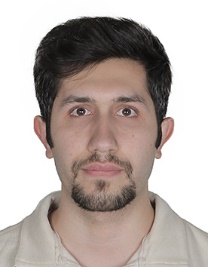
\includegraphics[width=1in,height=1.25in,clip,keepaspectratio]{Figures/authors/Younesi.jpg}}]{Abolfazl Younesi}(Student Member, IEEE)
is currently pursuing a PhD at the University of Innsbruck. He is a member of the Distributed and Parallel Systems Group (DPS) at the Department of Computer Science. He is working on European Union-funded projects. His research interests include Distributed Systems, Stream Processing, Federated Learning, and the Computing Continuum, with a focus on intelligent resource management, time-sensitive scheduling, and compute optimization.
\end{IEEEbiography}
\vspace{-1cm}
\begin{IEEEbiography}[{
\includegraphics[width=1in,height=1.25in,clip,keepaspectratio]{Figures/authors/SP.jpg}}]{Stefan Pedratscher} received the M.Sc. degree in Computer Science from the University of Innsbruck, Austria, in 2021. He is currently pursuing the Ph.D. degree with the Distributed and Parallel Systems Group at the same institution. His research interests include serverless computing and high-performance stream processing across the edge–cloud continuum.

\end{IEEEbiography}
\vspace{-1cm}

\begin{IEEEbiography}[{
\includegraphics[width=1in,height=1.25in,clip,keepaspectratio]{Figures/authors/citations.jpeg}}]{Zahra Najafabadi Samani}
received her PhD degree from the University of Klagenfurt, Austria, in 2023. She has been a postdoctoral researcher and university assistant since 2023 in the Distributed and Parallel Systems group at the University of Innsbruck, Austria. She has actively contributed to several national and European Union projects. Her main research interests include resource management and performance optimization in cloud, fog, and edge computing.
\end{IEEEbiography}
\vspace{-1cm}

\begin{IEEEbiography}[{
\includegraphics[width=1in,height=1.25in,clip,keepaspectratio]{Figures/authors/juan.jpg}}]{Juan Aznar Poveda} 
received his Ph.D. degree in Telecommunications Engineering from the Technical University of Cartagena, Spain, in 2022. He was awarded the prize “Liberalization of Telecommunications” (national level) for the best B.Sc. thesis in 2016. He is currently a postdoctoral researcher at the Distributed and Parallel Systems group of the University of Innsbruck, Austria. His research interests include Distributed Systems, Cyber-Physical Systems (CPS), Internet of Things, Artificial Intelligence, and Wireless networks and communications.
\end{IEEEbiography}
\vspace{-1cm}

\begin{IEEEbiography}[{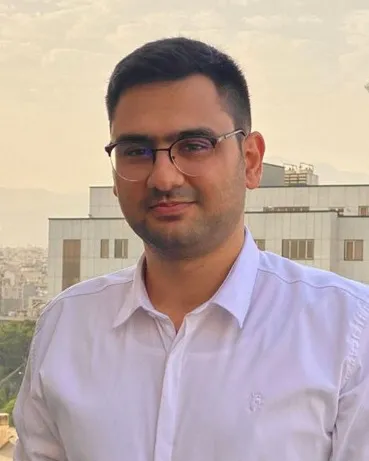
\includegraphics[width=1in,height=1.25in,clip,keepaspectratio]{Figures/authors/Photo.jpg}}]{Siavash Razmi}  is currently pursuing a PhD in Computer Science at the University of Innsbruck. He is a member of the Distributed and Parallel Systems (DPS) Group at the Department of Computer Science, working on EU-funded research projects. His research focuses on federated learning and graph neural networks for anomaly detection, root cause analysis, and fault detection in distributed and cloud–edge systems. His broad interests are representation learning, anomaly detection in graph neural networks, and time-series analysis.

\end{IEEEbiography}
\vspace{-1cm}


\begin{IEEEbiography}[{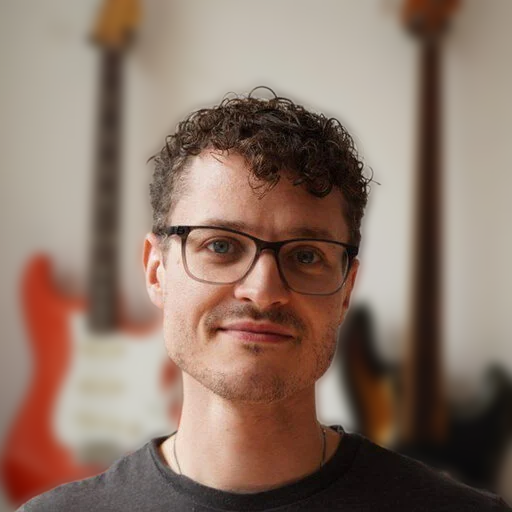
\includegraphics[width=1in,height=1.25in,clip,keepaspectratio]{Figures/authors/Marlon-Etheredge.jpg}}]{Marlon Etheredge} received the M.Sc. degree in Artificial Intelligence from Utrecht University, The Netherlands, in 2016. He is currently pursuing a Ph.D. degree with the Distributed and Parallel Systems Group at the University of Innsbruck, Austria. His research interests include programming paradigms and runtime systems for distributed applications operating across the cloud–edge–IoT continuum.
\end{IEEEbiography}
\vspace{-1cm}


\begin{IEEEbiography}[{
\includegraphics[width=1in,height=1.25in,clip,keepaspectratio]{Figures/authors/1669364923872.jpg}}]{Philipp Gschwandtner}  is head of the Research Center HPC at the University of Innsbruck, Austria. He graduated from the Doctoral Programme Computational Interdisciplinary Modelling in Computer Science, focusing on performance and energy analysis and optimization of parallel programs. His main interests lie in research and training in HPC and scientific computing, including adjacent topics such as programming model design, runtime systems, or compiler research. He collaborated in multiple national and international projects (e.g., FFG UMUGUC, H2020 LIGATE, H2020 PRACE-6IP, H2020 AllScale, CHIST-ERA GEMSCLAIM, FWF/DST EASE) and co-organized multiple international conferences.
\end{IEEEbiography}
\vspace{-1cm}

\begin{IEEEbiography}[{
\includegraphics[width=1in,height=1.25in,clip,keepaspectratio]{Figures/authors/petert_crop.jpg}}]{Peter Thoman} 
is an associate professor with the Distributed and Parallel Systems group at the University of Innsbruck, and CTO and co-founder of PH3 GmbH. He is one of the original developers and designers of the Celerity runtime system for accelerator clusters and the Insieme C++ research compiler, and was involved in multiple international research projects in this capacity. Peter’s research interests include API and runtime system design for parallelism, accelerator computing, fine-grained task parallelism, and compiler-supported optimizations. He is a representative of the University of Innsbruck at Khronos and a member of the SYCL working group.
\end{IEEEbiography}

\vspace{-1cm}

\begin{IEEEbiography}[{
\includegraphics[width=1in,height=1in,clip,keepaspectratio]{Figures/authors/balis.jpg}}]{Bartosz Balis} 
received the M.Sc. degree from the AGH University of Krakow and Jagiellonian University, and the Ph.D. and D.Sc. (Habilitation) degrees in computer science from the AGH University of Krakow. He is an Associate Professor with the Faculty of Computer Science, AGH University of Krakow; and a Senior Postgraduate Researcher with the Sano Centre for Computational Medicine. He is also involved in the ALICE experiment with CERN. He is the coauthor of more than 100 international peer-reviewed scientific publications. His research interests include scientific workflow management, data science, cloud computing, and distributed computing. He has participated in national and EU-funded research projects, such as CrossGrid, CoreGRID, PL-Grid, K-Wf Grid, ViroLab, Gredia, UrbanFlood, PaaSage, ISMOP, WATERLINE, InSilicoWorld, and CLOUDSTARS. He has been a member of conference program and organizing committees, including the Euro-Par 2020 Workshops (the General Co-chair), the IEEE/ACM SC18 Birds of a Feather Planning Committee, and the IEEE/ACM SC16 Workshops Planning Committee.
\end{IEEEbiography}

\begin{IEEEbiography}[{
\includegraphics[width=1in,height=1.25in,clip,keepaspectratio]{Figures/authors/thomas.jpg}}]{Thomas Fahringer}(Member, IEEE) received the PhD degree from the Vienna University of Technology in 1993. He has been a full professor of computer science with the Institute of Computer Science, University of Innsbruck, Austria, since 2003. His main research interests include software architectures, programming paradigms, compiler technology, performance analysis, and prediction for parallel and distributed systems.
\end{IEEEbiography}


\vfill

\end{document}


